\chapter{Definitions}

Reader may already know some basic definitions of polyhedrons and polytopes and also might be familiar with some basic theorems and characterization. But in the other case we will introduce some of these basics one more time. Also note that the main part is that we are considering somewhat basic linear program.

$$
\begin{aligned}
	\max c^{T} x \\
	A x \leq b
\end{aligned}
$$

\noindent Where we are considering a finite number of linear inequalities.

\section{Polyhedra and Polytopes}

The polyhedron created by such linear program is usually called \hpoly{hedron}. But we will formulate it more precisely.

\begin{defn}
	\hpoly{hedron} is prescribed as $\{x | A x \leq b\}$ where $A \in \R^{m \times n}$ and $b \in \R^{n}$.
\end{defn}

\begin{defn}[Minkowski sum]
	Minkowski sum of two sets $A,B$ denoted by $A \msum B$ is $\{a + b | a \in A, b \in B\}$.
\end{defn}

\begin{defn}[Combinations]
	Let $V$ be a finite set, then by the following statements

	\begin{enumerate}
			\item $x = \sum_{v_{i} \in V} \lambda_{i} v_{i}, \lambda_{i} \in \R${}
			\item $1 = \sum_{v_{i} \in V} \lambda_{i}$
			\item $0 \leq \lambda_{i}$
	\end{enumerate}

	\noindent we will define:

	\begin{itemize}
			\item Linear combination $\lin(V)$ as 1.
			\item Affince combination $\aff(V)$ as 1. and 2.
			\item Conic combination $\cone(V)$ as 1. and 3.
			\item Convex combination $\conv(V)$ as 1., 2. and 3.
	\end{itemize}
\end{defn}

\begin{figure}[!ht]\centering
	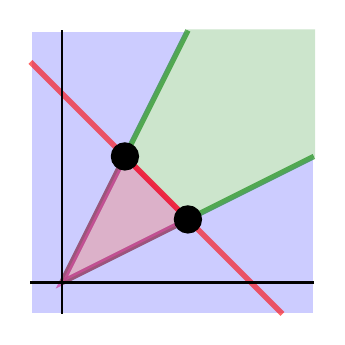
\begin{tikzpicture}[main/.style = {draw, circle, fill}, thick,
		comb/.style = {opacity = .6, line width = 2pt}, scale=.4]
			\draw[Blue!0, fill=Blue!20] (-1,-1) -- (-1,8) -- (8,8) -- (8,-1) -- cycle;
			\draw[Green!20, fill=Green!20] (0,0) -- (8,4) -- (8,8) -- (4,8) -- cycle;
			\draw[Green, comb] (4,8) -- (0,0);
			\draw[Green, comb] (8,4) -- (0,0);
			\draw[VioletRed, fill=VioletRed!50, comb] (0,0) -- (2,4) -- (4,2) -- cycle;
			\draw[Red, comb] (-1,7) -- (7,-1);
			\draw (-1,0) -- (8,0);
			\draw (0,-1) -- (0,8);
			\node[main] (1) at (4,2) {};
			\node[main] (2) at (2,4) {};
	\end{tikzpicture}
	\caption{Example of combinations, where $V$ are two points in $\R^{2}$, then we have their \textcolor{Blue}{linear combination}, \textcolor{Red}{affine combination}, \textcolor{Green}{conic combination} and \textcolor{VioletRed}{convex combination}.}
\end{figure}

\begin{defn}
	\vpoly{hedron} is defined as $\conv(V) \msum \cone(Y)$ where $V,Y$ are finite set of points.
\end{defn}

\begin{defn}
	Bounded-polyhedron is called \textbf{polytope}.
\end{defn}

This can be either visualized just by the definition or consider having a $n$-dimensional ball which is being cut by hyperplanes until no surface obtained by the ball itself persists.

\subsection{Examples of polytopes}

\subsubsection{Simplex}

This is a well known polytope which can be prescribed as follows. $k$-simplex is a convex combination of $k+1$ affine independent vertices.

\subsubsection{Cube}

Cube is even more known than the simplex. Already here we can see that it can be prescribed as \hpoly{tope} $\{x \in \R^{k} | 0 \leq x_{i} \leq 1\}$, but also as \vpoly{tope} $\conv(\{0,1\}^{k})$. This is quite essential, because we will see that \hpoly{hedra} and \vpoly{hedra} are equal.

\begin{figure}[!ht]\centering
	\begin{subfigure}{.45\textwidth}\centering
		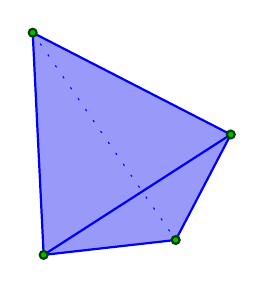
\begin{tikzpicture}
			[x={(0.454139cm, -0.658120cm)},
			y={(0.803660cm, 0.011660cm)},
			z={(-0.384562cm, -0.752823cm)},
			scale=2.000000,
			back/.style={loosely dotted, thin},
			edge/.style={color=blue!95!black, thick},
			facet/.style={fill=blue!95!black,fill opacity=0.400000},
			vertex/.style={inner sep=1pt,circle,draw=green!25!black,fill=green!75!black,thick}]
			\coordinate (-1.00000, 0.00000, 0.00000) at (-1.00000, 0.00000, 0.00000);
			\coordinate (0.00000, 0.00000, 1.00000) at (0.00000, 0.00000, 1.00000);
			\coordinate (0.00000, 1.00000, 0.00000) at (0.00000, 1.00000, 0.00000);
			\coordinate (1.00000, 0.00000, 0.00000) at (1.00000, 0.00000, 0.00000);
			\draw[edge,back] (-1.00000, 0.00000, 0.00000) -- (1.00000, 0.00000, 0.00000);
			\fill[facet] (0.00000, 1.00000, 0.00000) -- (-1.00000, 0.00000, 0.00000) -- (0.00000, 0.00000, 1.00000) -- cycle {};
			\fill[facet] (1.00000, 0.00000, 0.00000) -- (0.00000, 0.00000, 1.00000) -- (0.00000, 1.00000, 0.00000) -- cycle {};
			\draw[edge] (-1.00000, 0.00000, 0.00000) -- (0.00000, 0.00000, 1.00000);
			\draw[edge] (-1.00000, 0.00000, 0.00000) -- (0.00000, 1.00000, 0.00000);
			\draw[edge] (0.00000, 0.00000, 1.00000) -- (0.00000, 1.00000, 0.00000);
			\draw[edge] (0.00000, 0.00000, 1.00000) -- (1.00000, 0.00000, 0.00000);
			\draw[edge] (0.00000, 1.00000, 0.00000) -- (1.00000, 0.00000, 0.00000);
			\node[vertex] at (-1.00000, 0.00000, 0.00000)     {};
			\node[vertex] at (0.00000, 0.00000, 1.00000)     {};
			\node[vertex] at (0.00000, 1.00000, 0.00000)     {};
			\node[vertex] at (1.00000, 0.00000, 0.00000)     {};
		\end{tikzpicture}
		\caption{3 dimensional simplex}
	\end{subfigure}
	\begin{subfigure}{.45\textwidth}\centering{}
		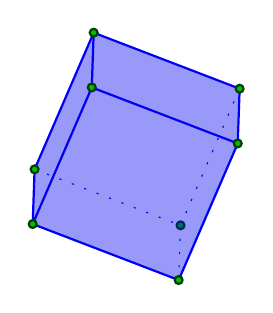
\begin{tikzpicture}
			[x={(0.926869cm, -0.355696cm)},
			y={(0.375194cm, 0.867588cm)},
			z={(-0.011997cm, -0.347523cm)},
			scale=2.000000,
			back/.style={loosely dotted, thin},
			edge/.style={color=blue!95!black, thick},
			facet/.style={fill=blue!95!black,fill opacity=0.400000},
			vertex/.style={inner sep=1pt,circle,draw=green!25!black,fill=green!75!black,thick}]
			\coordinate (0.00000, 0.00000, 0.00000) at (0.00000, 0.00000, 0.00000);
			\coordinate (0.00000, 0.00000, 1.00000) at (0.00000, 0.00000, 1.00000);
			\coordinate (0.00000, 1.00000, 0.00000) at (0.00000, 1.00000, 0.00000);
			\coordinate (0.00000, 1.00000, 1.00000) at (0.00000, 1.00000, 1.00000);
			\coordinate (1.00000, 0.00000, 0.00000) at (1.00000, 0.00000, 0.00000);
			\coordinate (1.00000, 0.00000, 1.00000) at (1.00000, 0.00000, 1.00000);
			\coordinate (1.00000, 1.00000, 0.00000) at (1.00000, 1.00000, 0.00000);
			\coordinate (1.00000, 1.00000, 1.00000) at (1.00000, 1.00000, 1.00000);
			\draw[edge,back] (0.00000, 0.00000, 0.00000) -- (1.00000, 0.00000, 0.00000);
			\draw[edge,back] (1.00000, 0.00000, 0.00000) -- (1.00000, 0.00000, 1.00000);
			\draw[edge,back] (1.00000, 0.00000, 0.00000) -- (1.00000, 1.00000, 0.00000);
			\node[vertex] at (1.00000, 0.00000, 0.00000)     {};
			\fill[facet] (1.00000, 1.00000, 1.00000) -- (0.00000, 1.00000, 1.00000) -- (0.00000, 0.00000, 1.00000) -- (1.00000, 0.00000, 1.00000) -- cycle {};
			\fill[facet] (1.00000, 1.00000, 1.00000) -- (0.00000, 1.00000, 1.00000) -- (0.00000, 1.00000, 0.00000) -- (1.00000, 1.00000, 0.00000) -- cycle {};
			\fill[facet] (0.00000, 1.00000, 1.00000) -- (0.00000, 0.00000, 1.00000) -- (0.00000, 0.00000, 0.00000) -- (0.00000, 1.00000, 0.00000) -- cycle {};
			\draw[edge] (0.00000, 0.00000, 0.00000) -- (0.00000, 0.00000, 1.00000);
			\draw[edge] (0.00000, 0.00000, 0.00000) -- (0.00000, 1.00000, 0.00000);
			\draw[edge] (0.00000, 0.00000, 1.00000) -- (0.00000, 1.00000, 1.00000);
			\draw[edge] (0.00000, 0.00000, 1.00000) -- (1.00000, 0.00000, 1.00000);
			\draw[edge] (0.00000, 1.00000, 0.00000) -- (0.00000, 1.00000, 1.00000);
			\draw[edge] (0.00000, 1.00000, 0.00000) -- (1.00000, 1.00000, 0.00000);
			\draw[edge] (0.00000, 1.00000, 1.00000) -- (1.00000, 1.00000, 1.00000);
			\draw[edge] (1.00000, 0.00000, 1.00000) -- (1.00000, 1.00000, 1.00000);
			\draw[edge] (1.00000, 1.00000, 0.00000) -- (1.00000, 1.00000, 1.00000);
			\node[vertex] at (0.00000, 0.00000, 0.00000)     {};
			\node[vertex] at (0.00000, 0.00000, 1.00000)     {};
			\node[vertex] at (0.00000, 1.00000, 0.00000)     {};
			\node[vertex] at (0.00000, 1.00000, 1.00000)     {};
			\node[vertex] at (1.00000, 0.00000, 1.00000)     {};
			\node[vertex] at (1.00000, 1.00000, 0.00000)     {};
			\node[vertex] at (1.00000, 1.00000, 1.00000)     {};
		\end{tikzpicture}
		\caption{3 dimensional cube}
	\end{subfigure}
\end{figure}

\subsubsection{Pyramids and other creations}

Also we will show us a simple way how to create new polytopes. That is imagine we have a polytope $P$ and put it in a higher dimension, then by adding one point above the $P$ and creating a convex hull of $P$ and the point we obtain a so called pyramid. We may also denote it as $\pyr(P)$. Similarly if we would take two points, where one is above and the second one is below the given $P$ we get bipyramid or $\bipyr(P)$.

Last creation we will show us right now is if we would take a parallel copy of the polytope $P$, that is to some other parallel hyperplane and connect these two together. This way we obtain a prism.

\begin{figure}[!ht]\centering
	\begin{subfigure}{.3\textwidth}\centering
			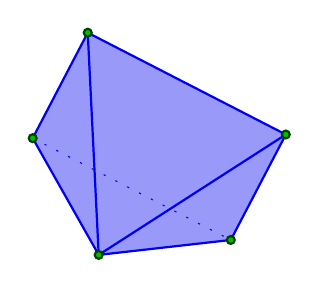
\begin{tikzpicture}
				[x={(0.454139cm, -0.658120cm)},
				y={(0.803660cm, 0.011660cm)},
				z={(-0.384562cm, -0.752823cm)},
				scale=2.000000,
				back/.style={loosely dotted, thin},
				edge/.style={color=blue!95!black, thick},
				facet/.style={fill=blue!95!black,fill opacity=0.400000},
				vertex/.style={inner sep=1pt,circle,draw=green!25!black,fill=green!75!black,thick}]
			\coordinate (-1.00000, 0.00000, 0.00000) at (-1.00000, 0.00000, 0.00000);
			\coordinate (0.00000, -1.00000, 0.00000) at (0.00000, -1.00000, 0.00000);
			\coordinate (0.00000, 0.00000, 1.00000) at (0.00000, 0.00000, 1.00000);
			\coordinate (0.00000, 1.00000, 0.00000) at (0.00000, 1.00000, 0.00000);
			\coordinate (1.00000, 0.00000, 0.00000) at (1.00000, 0.00000, 0.00000);
			\draw[edge,back] (0.00000, -1.00000, 0.00000) -- (1.00000, 0.00000, 0.00000);
			\fill[facet] (0.00000, 0.00000, 1.00000) -- (-1.00000, 0.00000, 0.00000) -- (0.00000, -1.00000, 0.00000) -- cycle {};
			\fill[facet] (0.00000, 1.00000, 0.00000) -- (-1.00000, 0.00000, 0.00000) -- (0.00000, 0.00000, 1.00000) -- cycle {};
			\fill[facet] (1.00000, 0.00000, 0.00000) -- (0.00000, 0.00000, 1.00000) -- (0.00000, 1.00000, 0.00000) -- cycle {};
			\draw[edge] (-1.00000, 0.00000, 0.00000) -- (0.00000, -1.00000, 0.00000);
			\draw[edge] (-1.00000, 0.00000, 0.00000) -- (0.00000, 0.00000, 1.00000);
			\draw[edge] (-1.00000, 0.00000, 0.00000) -- (0.00000, 1.00000, 0.00000);
			\draw[edge] (0.00000, -1.00000, 0.00000) -- (0.00000, 0.00000, 1.00000);
			\draw[edge] (0.00000, 0.00000, 1.00000) -- (0.00000, 1.00000, 0.00000);
			\draw[edge] (0.00000, 0.00000, 1.00000) -- (1.00000, 0.00000, 0.00000);
			\draw[edge] (0.00000, 1.00000, 0.00000) -- (1.00000, 0.00000, 0.00000);
			\node[vertex] at (-1.00000, 0.00000, 0.00000)     {};
			\node[vertex] at (0.00000, -1.00000, 0.00000)     {};
			\node[vertex] at (0.00000, 0.00000, 1.00000)     {};
			\node[vertex] at (0.00000, 1.00000, 0.00000)     {};
			\node[vertex] at (1.00000, 0.00000, 0.00000)     {};
		\end{tikzpicture}
		\caption{Pyramid}
	\end{subfigure}
	\begin{subfigure}{.3\textwidth}\centering
			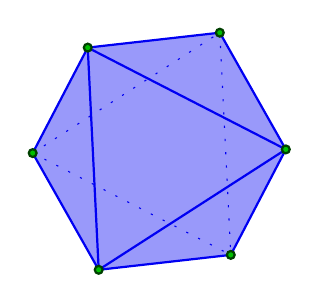
\begin{tikzpicture}
			[x={(0.454139cm, -0.658120cm)},
			y={(0.803660cm, 0.011660cm)},
			z={(-0.384562cm, -0.752823cm)},
			scale=2.000000,
			back/.style={loosely dotted, thin},
			edge/.style={color=blue!95!black, thick},
			facet/.style={fill=blue!95!black,fill opacity=0.400000},
			vertex/.style={inner sep=1pt,circle,draw=green!25!black,fill=green!75!black,thick}]
		\coordinate (-1.00000, 0.00000, 0.00000) at (-1.00000, 0.00000, 0.00000);
		\coordinate (0.00000, -1.00000, 0.00000) at (0.00000, -1.00000, 0.00000);
		\coordinate (0.00000, 0.00000, -1.00000) at (0.00000, 0.00000, -1.00000);
		\coordinate (0.00000, 0.00000, 1.00000) at (0.00000, 0.00000, 1.00000);
		\coordinate (0.00000, 1.00000, 0.00000) at (0.00000, 1.00000, 0.00000);
		\coordinate (1.00000, 0.00000, 0.00000) at (1.00000, 0.00000, 0.00000);
		\draw[edge,back] (0.00000, -1.00000, 0.00000) -- (0.00000, 0.00000, -1.00000);
		\draw[edge,back] (0.00000, -1.00000, 0.00000) -- (1.00000, 0.00000, 0.00000);
		\draw[edge,back] (0.00000, 0.00000, -1.00000) -- (1.00000, 0.00000, 0.00000);
		\fill[facet] (0.00000, 1.00000, 0.00000) -- (-1.00000, 0.00000, 0.00000) -- (0.00000, 0.00000, 1.00000) -- cycle {};
		\fill[facet] (0.00000, 0.00000, 1.00000) -- (-1.00000, 0.00000, 0.00000) -- (0.00000, -1.00000, 0.00000) -- cycle {};
		\fill[facet] (0.00000, 1.00000, 0.00000) -- (-1.00000, 0.00000, 0.00000) -- (0.00000, 0.00000, -1.00000) -- cycle {};
		\fill[facet] (1.00000, 0.00000, 0.00000) -- (0.00000, 0.00000, 1.00000) -- (0.00000, 1.00000, 0.00000) -- cycle {};
		\draw[edge] (-1.00000, 0.00000, 0.00000) -- (0.00000, -1.00000, 0.00000);
		\draw[edge] (-1.00000, 0.00000, 0.00000) -- (0.00000, 0.00000, -1.00000);
		\draw[edge] (-1.00000, 0.00000, 0.00000) -- (0.00000, 0.00000, 1.00000);
		\draw[edge] (-1.00000, 0.00000, 0.00000) -- (0.00000, 1.00000, 0.00000);
		\draw[edge] (0.00000, -1.00000, 0.00000) -- (0.00000, 0.00000, 1.00000);
		\draw[edge] (0.00000, 0.00000, -1.00000) -- (0.00000, 1.00000, 0.00000);
		\draw[edge] (0.00000, 0.00000, 1.00000) -- (0.00000, 1.00000, 0.00000);
		\draw[edge] (0.00000, 0.00000, 1.00000) -- (1.00000, 0.00000, 0.00000);
		\draw[edge] (0.00000, 1.00000, 0.00000) -- (1.00000, 0.00000, 0.00000);
		\node[vertex] at (-1.00000, 0.00000, 0.00000)     {};
		\node[vertex] at (0.00000, -1.00000, 0.00000)     {};
		\node[vertex] at (0.00000, 0.00000, -1.00000)     {};
		\node[vertex] at (0.00000, 0.00000, 1.00000)     {};
		\node[vertex] at (0.00000, 1.00000, 0.00000)     {};
		\node[vertex] at (1.00000, 0.00000, 0.00000)     {};
		\end{tikzpicture}
		\caption{Bipyramid}
	\end{subfigure}
	\begin{subfigure}{.3\textwidth}\centering{}
		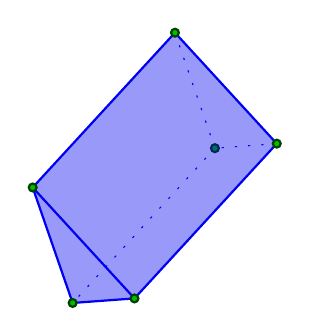
\begin{tikzpicture}
			[x={(0.181209cm, -0.523814cm)},
			y={(0.742124cm, -0.482509cm)},
			z={(-0.645302cm, -0.702000cm)},
			scale=1.400000,
			back/.style={loosely dotted, thin},
			edge/.style={color=blue!95!black, thick},
			facet/.style={fill=blue!95!black,fill opacity=0.400000},
			vertex/.style={inner sep=1pt,circle,draw=green!25!black,fill=green!75!black,thick}]
			\coordinate (-1.00000, 0.00000, 0.00000) at (-1.00000, 0.00000, 0.00000);
			\coordinate (-1.00000, 0.00000, 2.00000) at (-1.00000, 0.00000, 2.00000);
			\coordinate (0.00000, 1.00000, 0.00000) at (0.00000, 1.00000, 0.00000);
			\coordinate (0.00000, 1.00000, 2.00000) at (0.00000, 1.00000, 2.00000);
			\coordinate (1.00000, 0.00000, 0.00000) at (1.00000, 0.00000, 0.00000);
			\coordinate (1.00000, 0.00000, 2.00000) at (1.00000, 0.00000, 2.00000);
			\draw[edge,back] (-1.00000, 0.00000, 0.00000) -- (1.00000, 0.00000, 0.00000);
			\draw[edge,back] (0.00000, 1.00000, 0.00000) -- (1.00000, 0.00000, 0.00000);
			\draw[edge,back] (1.00000, 0.00000, 0.00000) -- (1.00000, 0.00000, 2.00000);
			\node[vertex] at (1.00000, 0.00000, 0.00000)     {};
			\fill[facet] (0.00000, 1.00000, 2.00000) -- (-1.00000, 0.00000, 2.00000) -- (-1.00000, 0.00000, 0.00000) -- (0.00000, 1.00000, 0.00000) -- cycle {};
			\fill[facet] (1.00000, 0.00000, 2.00000) -- (-1.00000, 0.00000, 2.00000) -- (0.00000, 1.00000, 2.00000) -- cycle {};
			\draw[edge] (-1.00000, 0.00000, 0.00000) -- (-1.00000, 0.00000, 2.00000);
			\draw[edge] (-1.00000, 0.00000, 0.00000) -- (0.00000, 1.00000, 0.00000);
			\draw[edge] (-1.00000, 0.00000, 2.00000) -- (0.00000, 1.00000, 2.00000);
			\draw[edge] (-1.00000, 0.00000, 2.00000) -- (1.00000, 0.00000, 2.00000);
			\draw[edge] (0.00000, 1.00000, 0.00000) -- (0.00000, 1.00000, 2.00000);
			\draw[edge] (0.00000, 1.00000, 2.00000) -- (1.00000, 0.00000, 2.00000);
			\node[vertex] at (-1.00000, 0.00000, 0.00000)     {};
			\node[vertex] at (-1.00000, 0.00000, 2.00000)     {};
			\node[vertex] at (0.00000, 1.00000, 0.00000)     {};
			\node[vertex] at (0.00000, 1.00000, 2.00000)     {};
			\node[vertex] at (1.00000, 0.00000, 2.00000)     {};
		\end{tikzpicture}
		\caption{Prism}
	\end{subfigure}
\end{figure}

\begin{thm}[Minkowski-Weyl]
	$P$ is \hpoly{hedron} $\iff$ it is a \vpoly{hedron}.
\end{thm}

\begin{proof}[Sketch of the proof]
	"$\Rightarrow$" We will gradually make the polyhedron more non-general and then consider a simple case. So WLOG:

	\begin{enumerate}
		\item $P$ is full-dimensional. Where dimension is defined as dimension of the smallest affine space containing it.
		\item $P$ is pointed, that is it does not contain a line. -- If it contains a line we can split it by an orthogonal hyperplane, inductively use Minkowski-Weyl theorem and then extend $Y$ by rays to both sides of the hyperplane. Use theorem \ref{pointed-P}.
		\item $V = \emptyset$ -- Use trick which is called \textbf{Homogenization} or \textbf{Homogenized cone} which is that $P : Ax \leq b$ create $P' : Ax - bz \leq 0$ and $z \geq 0$. So for $z = 1$ we have original $P$ and then for all others $z$ we have scaled copy of $P$. After this trick we use Minkowski-Weyl for this cone and create $V$ by the points for which $z > 0$ and $Y$ from poitns for which $z = 0$.
		\item $P$ is a polytope. And with tha we use claim \ref{polytope}.
	\end{enumerate}

	"$\Leftarrow$" Set $P = \{x | x = \sum \lambda_{i} x_{i}, 1 = \sum \lambda_{i}, 0 \leq \lambda_{i}\}$ which is a \hpoly{tope}. By also using Fourier Monskin split to positive, 0 and negative koeficients.
\end{proof}

\begin{thm}
	$P$ is a pointed $\iff$ it has an extreme point.
	\label{pointed-P}
\end{thm}

\begin{proof}
	If there is a line and we have extreme point we can shift the line so it goes through the extreme point. But now the line representing the optimization function is either parallel hence it is not an extreme point or not parallel which also implies it is not an extreme point.
\end{proof}

\begin{claim}
Lets have polytope $P = \{x | A x \leq b\}$ and $V$ be the set of extreme point of $P$. Then $P = \conv(V)$.
	\label{polytope}
\end{claim}

\begin{proof}
	"$P \supseteq \conv(V)$" Is easy. So see "$P \subseteq \conv(V)$". Suppose it is not true. Take any such $x$ and find a hyperplane separating $\conv(V)$ and $x$ which can be done by Hyperplane separation lemma (that is choosing shortest segment and creating an orthogonal hyperplane between them). Then the optimum of the direction set by the norm of this hyperplane gives an extreme point, which is a contradiction.
\end{proof}

From the main theorem we may see that from mathematical perspective both \hpoly{hedrons} and \vpoly{hedrons} are the same. But for computer scientists it is pretty much the opposite. Consider solving an LP. Given linear inequalities it takes some time to solve it, but if we have all vertices we can just check every one of them if it is optimum. Also iff we would like to see an intersection of two polytopes $P,Q$ it is the opposite. That is we can just add all inequalities together and obtain their intersection. On the other hand for convex points it is known to be NP hard.

\begin{fact}
	For polytope $P \subseteq \R^{d}$ given by $n$ inequalitites it has $\leq n^{\lfloor d/2 \rfloor}$ vertices.
\end{fact}
